\chapter{Messergebnisse}

Dieses Kapitel be\-han\-delt die Mess\-er\-geb\-nis\-se, welche mit dem zu\-vor be\-schrie\-be\-nen System erzielt wurden. Dabei wird von verschiedenen Sze\-narien aus\-ge\-gang\-en, welche die jeweiligen Vor- und Nach\-teile der zwei Sy\-stem\-en zum Ausdruck bringen sollen. 

\section{Laborumgebung}

Alle Messergebnisse stammen aus einer La\-bor\-um\-gebung, mit fol\-gen\-den Ei\-gen\-schaf\-ten:

Dieses Kapitel be\-handelt die Mes\-ser\-ge\-bis\-se, welche mit dem zuvor be\-schrie\-benen System erzielt wurden. Dabei wird von verschiedenen Szenarien ausgegangen, welche die jeweiligen Vor- und Nachteile der zwei Systemen zum Ausdruck bringen sollen. \newline
Alle Mes\-ser\-ge\-bnis\-se stam\-men aus einer Labor\-umgebung, mit folgenden Ei\-gen\-schaf\-ten:

\begin{itemize}
\item Alle Testrechner, Server wie Client, besitzen folgende Hardware:
\begin{itemize}
\item Prozessor: Intel Xeon CPU X3450, 8 x 2.67Ghz
\item Speicher: RAM 8GB
\item Netzwerkkarte: Intel 82578DM Gigabit Network Card
\end{itemize}
\item Folgende Betriebssysteme wurden während den Messungen verwendet:
\begin{itemize}
\item Server: Ubuntu, Version 11.10
\item Auf beiden Clients: Fedora Linux, Release 16
\end{itemize}
\item Die Netzwerkinfrastruktur im Laborraum ist kaum belastet, daher nur durch den gebräuchlichen Leerlaufverkehr(STP, ARP usw.)
\item Die Hardware-Ressourcen der Rechner, auf welchen die Applikation getestet wird, sind ausschliesslich nur durch die Applikation belegt und durch einzelne, übliche Prozesse vom  Betriebsystem.
\end{itemize}

\section{Testvorgaben}
Die in dieser Arbeit ausgewiesenen Zahlen wurden alle in der Laborumgebung gemessen. Dabei wurde für jeden TestCase die Anzahl der Clients schrittweise von zwei bis acht Clients erhöht. Jeder Testlauf mit der gleichen Anzahl Clients, wurde drei Mal durchgeführt, um einen exakten Mittelwert der Ergebnisse ausweisen zu können. Drei Testdurchläufe pro Scenario und Clientanzahl wurden aufgrund der sehr nahe liegenden Ergbnisse der Testdurchläufe als genügend eingestuft. Wären die einzelnen Ergebnisse der Durchläufe extrem unterschiedlich, hätten fünf oder mehr Durchläufe stattfinden müssen.

\section{Testergebnisse}
In den folgenden Kapiteln werden die getesteten Scenarios und deren Ergebnisse gezeigt. 

\subsection{Nur lesende Clients}
\subsubsection{Szenario Code}
Dieser TestCase sieht folgendermassen aus:
\begin{lstlisting}[breaklines=true]
<?xml version='1.0' encoding='UTF-8'?>
<TestRun>
  <TestCase
    ClientSystemUnderTest="ch.hsr.objectCaching.rmiWithCacheClient.RMIwithCacheClientSystem"
    ServerSystemUnderTest="ch.hsr.objectCaching.rmiWithCacheServer.RMIWithCacheServerSystem">
    <Account balance="1"></Account>
      <Scenario id="1">
        <ActionSequence>
          <Read count="250"></Read>
	</ActionSequence>
      </Scenario>
  </TestCase>
</TestRun>
\end{lstlisting}

\subsubsection{Szenariobeschreibung}
Bei diesem Testcase führen alle Clients die gleichen Operationen aus. Alle Clients lesen das Objekt auf dem Server genau 250 Mal. Das Account-Objekt wird mit dem Wert "1" initialisiert, welcher bis zum Schluss unverändert bleiben wird. \newline
Zu erwarten ist ein enormer Geschwindigkeitsvorteil des Cache-Systems. Da bei diesem Testcase keine Schreiboperationen getätigt werden, wird ein Update der Clients nie nötig sein. Dadurch muss der Cache nur beim ersten Lesezugriff aktualisiert werden und die weiteren Lesezugriffe können lokal auf dem Rechner abgewickelt werden. Daher scheint es nur logisch, dass das Cache-System um einiges schneller ist. \newline
Weiter soll aufgezeigt werden, dass das Cache-System zumindest bei nur Lesezugriffen um einiges besser skaliert, als das System ohne Cache. Es wird also erwartet, dass beim Cache-System die Lesezugriffe gleich schnell bleiben, egal wieviele Clients beim Testdurchlau involviert sind. Beim System ohne Cache jedoch, wird eine lineare Verschlechterung der Zugriffszit erwartet.

\subsubsection{Ergebnisse RMI-Only System}

Die folgende Tabelle stellt die Messergebnisse des RMI-Only-System dar:  \newline


\resizebox{6cm}{!} {
\begin{tabular*}{6.5cm}[]{l l l l l l}
Legende&2Clients&3Clients&4Clients&5Clients\\
\cline{1-5}
setBalance&0&0&0&0\\
getBalance&86.182&89.502273&91.313&94.490998\\
Konfliktanzahl&0&0&0&0\\
TotalTime(with Delays)&21546.54&22376.494&22829.21&23623.678\\
PureOperationTime&21545.686&22375.568&22828.264&23622.749\\
\end{tabular*} }
\newline
\newline

\resizebox{6cm}{!} {
\begin{tabular*}{6.5cm}[]{l l l l}
Legende&6Clients&7Clients&8Clients\\
\cline{1-4}
setBalance&0&0&0\\
getBalance&98.381525&105.14788&120.2947\\
Konfliktanzahl&0&0&0\\
TotalTime(with Delays)&24596.331&26287.93&30074.669\\
Pure Operation Time&24595.381&26286.969&30073.691\\
\end{tabular*} } \newline

Diese Zahlen sind Durchschnittswerte von drei Messungen. Die genauen Messdaten können im Anhang gefunden werden. Die folgende Grafik zeigt den Verlauf des Zeitaufwandes mit einer steigenden Anzahl Clients von zwei bis acht Clients:
\begin{figure}[H]
\begin{center}
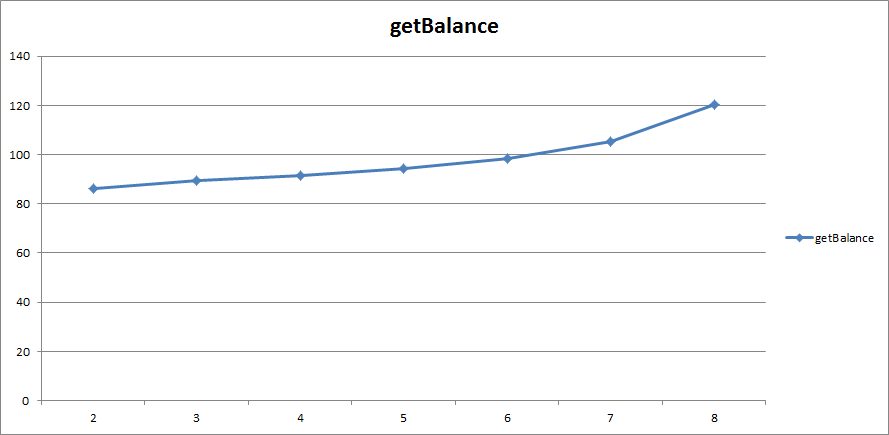
\includegraphics[scale=0.6]{images_MessErgebnisse/getBalance_RMI.png}
\end{center}
\end{figure}
Es wird schnell ersichtlich, dass das System mit einer steigenden Anzahl Clients langsamer wird. Dies erscheint durchaus logisch, da jeder getBalance-Aufruf an den Server gesendet wird. Wird der Server nun von mehreren Clients angefragt, verschlechtern sich auch dessen Antwortzeiten, was eine verlangsamung des Aufrufs zur Folge hat.

\subsubsection{Ergebnisse RMI-Only mit Cache System}

In der folgenden Tabelle werden die Messdaten des Cache-Systems dargestellt: \newline


\resizebox{6cm}{!} {
\begin{tabular*}{6.5cm}[]{l l l l l l}
Legende&2Clients&3Clients&4Clients&5Clients\\
\cline{1-5}
setBalance&0&0&0&0\\
getBalance&0.2889&0.2874&0.2852&0.2984\\
Konfliktanzahl&0&0&0&0\\
TotalTime(with Delays)&73.0871&72.5819&72.0394&75.4229\\
PureOperationTime&72.2497&71.8551&71.3044&74.6033\\
\end{tabular*} }
\newline
\newline

\resizebox{6cm}{!} {
\begin{tabular*}{6.5cm}[]{l l l l}
Legende&6Clients&7Clients&8Clients\\
\cline{1-4}
setBalance&0&0&0\\
getBalance&0.3011&0.3201&0.2810\\
Konfliktanzahl&0&0&0\\
TotalTime(with Delays)&76.0142&80.8389&71.0016\\
Pure Operation Time&75.2893&80.0410&70.2629\\
\end{tabular*} } \newline

Diese Zahlen sind wiederum Durchschnittswerte.  In der folgenden Grafik werden die durchschnittlichen Zeiten der \texttt{getBalance()}-Methode in Abhängigkeit der Anzahl Clients ausgegeben:

\begin{figure}[H]
\begin{center}
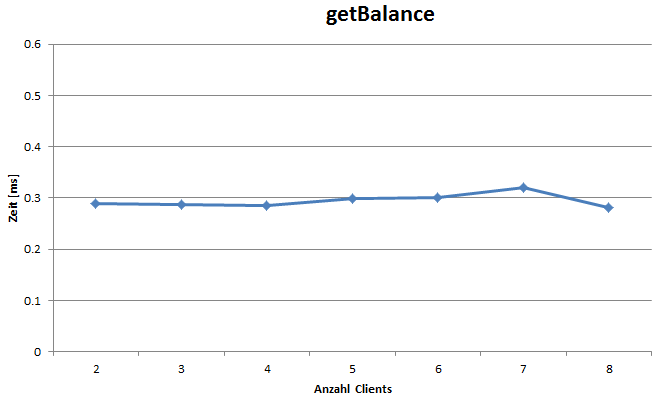
\includegraphics[scale=0.6]{images_MessErgebnisse/getBalance_03ms.png}
\end{center}
\end{figure}

Damit die Grafik einen Sinn ergibt, mussten die Zeiten auf der Y-Achse angepasst werden. Hätte man die Skala aus dem RMI-Only-System übernommen, wäre auf der Grafik nur eine Linie ersichtlich. Es muss dennoch bemerkt werden, dass bei dieser Grafik die Skala auf der Y-Achse extrem klein ist und Messunterschiede, wenn auch nur Minimale, in dieser Grafik stark zum tragen kommen. Ein Vergleich mit der vorhergehenden Grafik des RMI-Only-Systems ist also mit Vorsicht zu geniessen.
\newline Aus der Grafik wird ersichtlich, dass bei nur lesenden Zugriffen das System perfekt skaliert. Die Werte betragen circa alle, egal wieviele Clients beteiligt sind, 0.3ms. Anzunehmen ist, dass noch viele weitere Clients dazugeschaltet werden könnten, ohne dass die Zugriffszeit markant zunehmen würde.


\subsubsection{Interpretation}

Vergleicht man die Messergebnisse der zwei Systeme miteinander, fallen zwei Merkmale auf:
\begin{itemize}
\item Jeder einzelne getBalance-Aufruf dauert beim RMI-Only-System extrem viel länger
\item Das Cache-System skaliert viel besser als das RMI-Only-System
\end{itemize}

Da jeder getBalance-Aufruf zum Server, das heisst über das Netzwerk, übertragen werden muss, ist es logisch, dass das System im Durchschnitt viel langsamer ist. Beim Cache-System wird nur der erste Aufruf zum Server übertragen, alle folgenden Aufrufe werden lokal aus dem Cache beantwortet. Dies erklärt den enormen Geschwindigkeitsvorteil des Cache-Systems bei jedem einzelnen Aufruf. \newline
Weiter skaliert das Cache-System bei diesem Testcase um einiges besser. Dadurch, dass bei steigender Anzahl Clients auch immer mehr Clients ein Update erhalten müssen, hätte man auch eine leichte Steigung der Messwerte beim Cache-System erwarten können. Da die Werte aber so klein sind und die Messmethode mit der in Java implementierten Funktion \texttt{nanoTime()} gemacht wurde, können kleine Ungenauigkeiten in diesem Bereich nicht ganz ausgeschlossen werden. Es kann also durchaus sein, dass das Cache-System bei einer steigenden Anzahl Clients eine linear, leicht ansteigende Gerade zeigen würde, dies aber durch die Ungenauigkeiten beim Messen nicht genau abgebildet wird. Es bleibt auf jeden Fall zu beachten, dass das Cache-System wunderbar skaliert und man den Testcase mit einer vielzahl der Clients durchführen könnte, ohne grosse Geschwindigkeitseinbussen in Kauf nehmen zu müssen. \newline
Auf der anderen Seite skaliert das RMI-Only-System weitaus schlechter. Bei der Erhöhung der Clients von vier bis acht, als rund eine Verdopplung der CLients, wächst die durchschnittliche Zeit zum Ausführen der getBalance-Methode um etwa 30ms. Dies entspricht einem Drittel der Zeit, welche ein \texttt{getBalance()}-Aufruf bei vier Clients benötigt. Würde man die Anzahl Clients noch verdoppeln oder sogar verdreifachen, würde die benötigte Zeit zum Ausführen der \texttt{getBalance()}-Methode wohl bald eine Schmerzgrenze der Wartezeiten durchbrechen.


\subsection{Ein schreibender, mehrere lesende Clients}
\subsubsection{Szenario Code}
Das Szenario ist wie folgt aufgebaut:
\begin{lstlisting}
<?xml version='1.0' encoding='UTF-8'?>
<TestRun>
  <TestCase
    ClientSystemUnderTest="ch.hsr.objectCaching.rmiWithCacheClient.RMIwithCacheClientSystem"
    ServerSystemUnderTest="ch.hsr.objectCaching.rmiWithCacheServer.RMIWithCacheServerSystem">
      <Account balance="1"></Account>
        <Scenario id="1">
	  <ActionSequence>
	    <Increment count="900" delay="0" factor="1.1"></Increment>
	  </ActionSequence>
	</Scenario>
	<Scenario id="2">
	  <ActionSequence>
	    <Read count="3000" delay="100"></Read>
	  </ActionSequence>
	</Scenario>
	<Scenario id="3">
	  <ActionSequence>
	    <Read count="3000" delay="100"></Read>
	  </ActionSequence>
	</Scenario>
\end{lstlisting}

Das Szenario ist nicht abschliessend dargestellt, da sich nun bis zum Szenario mit der Id acht, die Szenariodefinitionen wiederholen. Der erste in der Clientliste eingetragene Client, wird immer den schreibenden Auftrag bekommen. Die anderen eins bis sieben Clients werden nur den Auftrag bekommen zu lesen. \newline
Für diesen Testcase wurde bei der Leseaktion extra noch ein Delay eingebaut. Die Clients müssen so lange lesen, wie der schreibende Client am arbeiten ist. Wären die lesenden Clients schon vor dem schreibenden Client fertig, würden sie sich herunterfahren und keine Updates mehr erhalten. Dies würde den Testcase verfälschen und somit nutzlos machen. Damit nun keine Million Reads angegeben werden mussten, wurde ein Delay eingebaut, damit die Clients lange genug aktiv bleiben. 
\subsubsection{Szenariobeschreibung}
In diesem Szenario geht es darum, dass nur ein Client den Balance-Wert erhöht und alle anderen Clients diesen Wert lesen. Beim RMI-Only-System wird bei steigender Anzahl Clients der Verkehr zum Server hin zunehmen. Es ist zu erwarten, dass durch diese Erhöhung die \texttt{SetBalance()}-Aufrufe bei steigender Anzahl Clients langsamer werden. \newline
Beim Cache-System ist wiederum auch eine kleine Steigung der Messwerte zu erwarten, da bei mehreren aktiven Clients, bei einer Änderung des Balance-Wertes, auch mehr Updates verschickt werden müssen. Dieser Testcase soll also zeigen, wie die Update-Funktion der Client-Caches skaliert, daher, ob das System bei acht Clients langsamer ist, als wenn nur zwei Clients beteiligt sind. \newline
Die folgende Auswertung der Messresultate beschränkt sich auf den schreibenden Client. Es soll ja untersucht werden, ob und wie stark sich eine steigende Anzahl lesender Clients auf die Schreibdauer eines Clients auswirkt. 

\subsubsection{Ergebnisse RMI-Only System}

Die Messwerte des schreibenden CLientss mit dem RMI-Only System sehen wie folgt aus: \newline


\resizebox{6cm}{!} {
\begin{tabular*}{6.5cm}[]{l l l l l l}
Legende&2Clients&3Clients&4Clients&5Clients\\
\cline{1-5}
setBalance&79.8705&79.9517&79.8211&79.8587\\
getBalance&80.1249&80.1400&80.1149&80.1421\\
Konfliktanzahl&0&0&0&0\\
TotalTime(with Delays)&80003.5573&80051.6692&79973.7976&80006.2888\\
PureOperationTime&79997.7365&80045.9110&79968.0607&80000.4531\\
\end{tabular*} }
\newline
\newline

\resizebox{6cm}{!} {
\begin{tabular*}{6.5cm}[]{l l l l}
Legende&6Clients&7Clients&8Clients\\
\cline{1-4}
setBalance&79.9147&79.8760&80.0812\\
getBalance&80.1332&80.1246&80.2016\\
Konfliktanzahl&0&0&0\\
TotalTime(with Delays)&80029.7826&80006.1374&80105.9440\\
Pure Operation Time&80024.0096&80000.3550&80100.1449\\
\end{tabular*} } \newline

Die Ergebnisse der \texttt{setBalance()}-Aurufe werden in dieser Abbildung grafisch dargestellt:

\begin{figure}[H]
\begin{center}
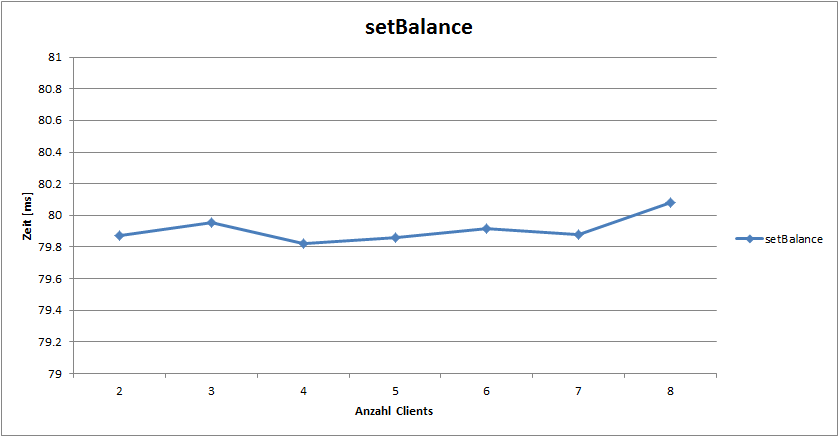
\includegraphics[scale=0.6]{images_MessErgebnisse/incrementAndReadRMI.png}
\end{center}
\end{figure}

Erstaundlicherweise skaliert das RMI-Only-System sehr gut. Die Werte für einen schreibenden Zugriff bleiben in etwa immer gleich. Anscheinend wurde das System etwas unterschätzt, denn augenscheinlich hätte man noch weit mehr Rechner lesen lassen können, ohne dass man eine Verlangsamung registriert hätte.


\subsubsection{Ergebnisse RMI-Only mit Cache System}

Folgende Tabelle zeigt die Messergebnisse des schreibenden Clients mit dem Cache-System: \newline


\resizebox{6cm}{!} {
\begin{tabular*}{6.5cm}[]{l l l l l l}
Legende&2Clients&3Clients&4Clients&5Clients\\
\cline{1-5}
setBalance&88.75211&88.7898&88.6036&88.6205\\
getBalance&0.1837&0.1845&0.1855&0.1842\\
Konfliktanzahl&0&0&0&0\\
TotalTime(with Delays)&80144.6425&80149.5192&79982.6941&80025.9731\\
PureOperationTime&80131.1769&80136.1886&79969.4380&80012.8222\\
\end{tabular*} }
\newline
\newline

\resizebox{6cm}{!} {
\begin{tabular*}{6.5cm}[]{l l l l}
Legende&6Clients&7Clients&8Clients\\
\cline{1-4}
setBalance&88.6558&88.7662&88.9202\\
getBalance&0.1895&0.1803&0.1925\\
Konfliktanzahl&0&0&0\\
TotalTime(with Delays)&80003.7567&80093.1801&80244.8572\\
Pure Operation Time&79990.5427&80081.5939&80231.3191\\
\end{tabular*} } \newline

In der folgenden Grafik ist der Verlauf der Messwerte der \texttt{setBalance()}-Aufrufe des schreibenden Clients zu sehen:
\begin{figure}[H]
\begin{center}
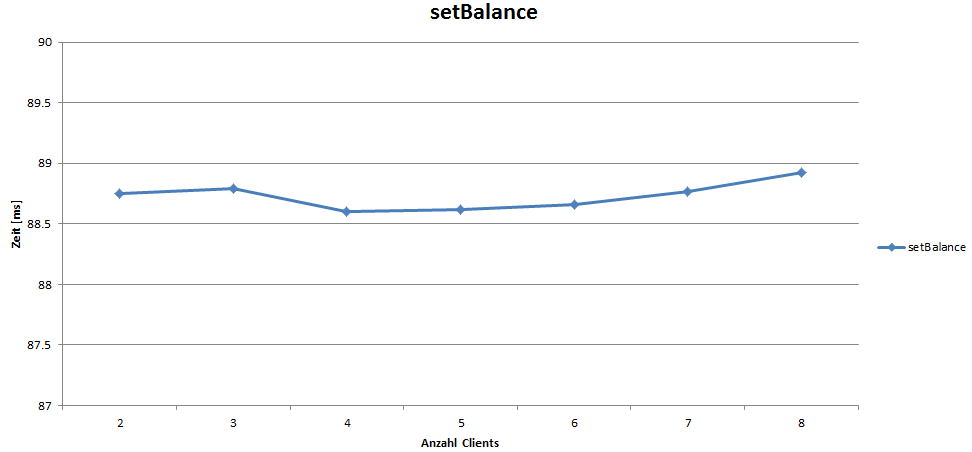
\includegraphics[scale=0.6]{images_MessErgebnisse/incrementAndReadCache.png}
\end{center}
\end{figure}

Wieder Erwarten steigt die gemessene Zeit mit zunehmenden Clients beim \texttt{setBalance()}-Aufruf nicht an. Die gemessene Zeit bleibt circa immer gleich, was darauf schliessen lässt, dass das Cache-System prima skaliert. Es scheint, als könnte man noch einige Clients mehr lesen lassen,  ohne eine spürbare Verlangsamung in Kauf nehmen zu müssen.

\subsubsection{Interpretation}

Dass das Cache-System bei diesem Testcase so gut skaliert war eigentlich zu erwarten. Mit einem leichten Anstieg der Messwerte wurde gerechnet, doch auch diese blieb ansich aus. Mit dem Problem der Zeitmessung in Java im Hinterkopf, kann man sagen, dass \texttt{setBalance()}-Aufrufe immer gleich schnell sind, egal, ob zwei oder acht Clients über den neuen Betrag des Balance-Wertes benachrichtigt werden müssen.\newline
Erstaundlicherweise skaliert jedoch auch das RMI-Only-System sehr gut. Die Werte der \texttt{setBalance()}-Aufrufe sind im Durchschnitt sogar noch etwas tiefer als die Werte, welche mit dem Cache-System gemessen wurden. Natürlich sind die \texttt{getBalance()}-Werte um ein vielfaches höher als im verglichenen Cache-System, dies war jedoch aufgrund des im vorhergehenden Testcases gezeigten Mechanismuses zu erwarten.\newline
Abschliessend lässt sich zu diesem Testcase sagen, dass weder das eine, noch das andere System abfällt. Beide arbeiten stabil und fehlerlos und wenn man nur die \texttt{setBalance()}-Werte betrachtet auch fast gleich schnell. Der Nachteil des RMI-Only-System bleibt wie erwähnt, die langsamen \texttt{getBalance()}-Aufrufe.

\subsection{Nur schreibende Clients}
\subsubsection{Szenario Code}
Der XML-Code, welcher dieses Szenario beschreibt, ist hier zu sehen:
\begin{lstlisting}
<?xml version='1.0' encoding='UTF-8'?>
<TestRun>
  <TestCase
    ClientSystemUnderTest="ch.hsr.objectCaching.rmiWithCacheClient.RMIwithCacheClientSystem"
    ServerSystemUnderTest="ch.hsr.objectCaching.rmiWithCacheServer.RMIWithCacheServerSystem">
    <Account balance="1"></Account>
      <Scenario id="1">
	<ActionSequence>
	  <Increment count="1000" delay="0" factor="1.1"></Increment>
	</ActionSequence>
      </Scenario>
  </TestCase>
</TestRun>
\end{lstlisting}
\subsubsection{Szenariobeschreibung}
In diesem Testcase führt jeder Client 1000 Mal ein Increment auf den Balance-Wert aus. Ein Increment bedeutet den Wert zu lesen und ihn dann mit einem Faktor multipliziert wieder zu schreiben. \newline
Ziel dieses Szenarios ist zu zeigen, wie sich die zwei Systeme bei permanentem Schreibzugriff verhalten. Dieses Szenario stellt eine enorme Belastung für den Server dar, da er mit Anfragen geradezu bombadiert wird. Durch die vielen Anfragen wird das System auch eine längere Zeit arbeiten müssen und so zum Vorschein bringen, ob es stabil und über längere Zeit sicher und fehlerlos läuft. \newline
Bei steigender Anzahl Clients, wird es auch mehr Schreibzugriffe auf den Server geben. Diest führt zu mehr Netzwerkverkehr und vor allem zu mehr Last auf dem Server, welcher alle Anfragen beantworten muss. Aus diesen Gründen wird erwartet, dass beide Systeme mit steigender Anzahl Clients eine steigende Antwortzeit ausweisen werden. Durch die schnelleren Lesezugriffe des Cache-Systems, wird aber eben dieses System insgesamt schneller arbeiten und somit besser skalieren.\newline
Ein weiterer Vorteil des Cache-Systems wird sein, dass es durch die Implementierung von zwei Concurrency-Control Mechanismen zu weniger Konflikten kommen wird. Wenn man sich vor Augen führt, dass bei acht Clients mit je 1000 Schreibzugriffen insgesamt 8000 Schreibzugriffe stattfinden, wird dies wohl ein grosser Vorteil für das Cache-System sein. Es wird also erwartet, dass das Cache-System um einiges besser skaliert.

\subsubsection{Ergebnisse RMI-Only System}

Die Messerwerte des RMI-Only-Systems: \newline


\resizebox{6cm}{!} {
\begin{tabular*}{6.5cm}[]{l l l l l l}
Legende&2Clients&3Clients&4Clients&5Clients\\
\cline{1-5}
setBalance&88.75211&88.7898&88.6036&88.6205\\
getBalance&0.1837&0.1845&0.1855&0.1842\\
Konfliktanzahl&0&0&0&0\\
TotalTime(with Delays)&80144.6425&80149.5192&79982.6941&80025.9731\\
PureOperationTime&80131.1769&80136.1886&79969.4380&80012.8222\\
\end{tabular*} }
\newline
\newline

\resizebox{6cm}{!} {
\begin{tabular*}{6.5cm}[]{l l l l}
Legende&6Clients&7Clients&8Clients\\
\cline{1-4}
setBalance&88.6558&88.7662&88.9202\\
getBalance&0.1895&0.1803&0.1925\\
Konfliktanzahl&0&0&0\\
TotalTime(with Delays)&80003.7567&80093.1801&80244.8572\\
Pure Operation Time&79990.5427&80081.5939&80231.3191\\
\end{tabular*} } \newline

\subsubsection{Ergebnisse RMI-Only mit Cache System}

In der folgenden Tabelle sind die Werte des Cache-Systems dargestellt:\newline


\resizebox{6cm}{!} {
\begin{tabular*}{6.5cm}[]{l l l l l l}
Legende&2Clients&3Clients&4Clients&5Clients\\
\cline{1-5}
setBalance&104.2852&130.9624&247.2939&427.0246\\
getBalance&0.1346&0.1007&0.1014&0.0993\\
Konfliktanzahl&681.5&1532.2222&1916.5&2243.8\\
TotalTime(with Delays)&176070.64&331890.26&721508.42&1385805\\
PureOperationTime&176052.29&331868.2&721482.83&1385777\\
\end{tabular*} }
\newline
\newline

\resizebox{6cm}{!} {
\begin{tabular*}{6.5cm}[]{l l l l}
Legende&6Clients&7Clients&8Clients\\
\cline{1-4}
setBalance&648.4426&981.2542&1353.4886\\
getBalance&0.1008&0.0972&0.0907\\
Konfliktanzahl&2534.5&2871.3333&3254.7083\\
TotalTime(with Delays)&2303134&3782179&5761716\\
Pure Operation Time&2303103&3800575&5761681\\
\end{tabular*} } \newline

\subsubsection{Interpretation}

